\section{Societal Factors}

Different societal factors plays an important role when looking at the demographics of a pandemic. These factors are seen and described as important variables which directly affects the spreading of a virus. Generally speaking there are countless factors to consider, but these factors can all be categorised to give an overview of how big an impact these societal factors have on the spread of COVID-19. 

In regards to the spreading of COVID-19 and other pandemics, these factors can be summarised into the following:

\begin{itemize}
    \item Population density 
    \item Living conditions of an area
    \item Socioeconomic status 
    \item Sanitary facilities 
    \item Cultural aspect
\end{itemize}

Although we recognise the validity of the aforementioned factors, we will primarily argument that the population density is one of the more important factors. \citep{who_listings_nodate} In addition to the population density, the culture of a designated country or area is also to be considered, since the spreading of a virus is highly dependant on how we interact with each other - as an example, these cultural factors include greetings, social gatherings, how we socialise with family and colleagues for examples - countries with seemingly common demographics can vary in total COVID-19 infections depending on the culture of the society.\citep{fanelli_analysis_2020}

\subsubsection{Population Density}
Population density is an important factor to consider when estimating the spread of a virus, such as COVID-19. This is both in terms of the total number of contacts a person has as well as the total duration of the disease. \\
The population density has an effect that is proportional to the contact rate \citep{rocklov_high_2020} in terms of the total number of contacts. This means that it would take less time for the disease to spread in a densely populated area. This in turn ties into the population density's effect on the spread and decay duration.
\begin{figure}[H]
    \centering
    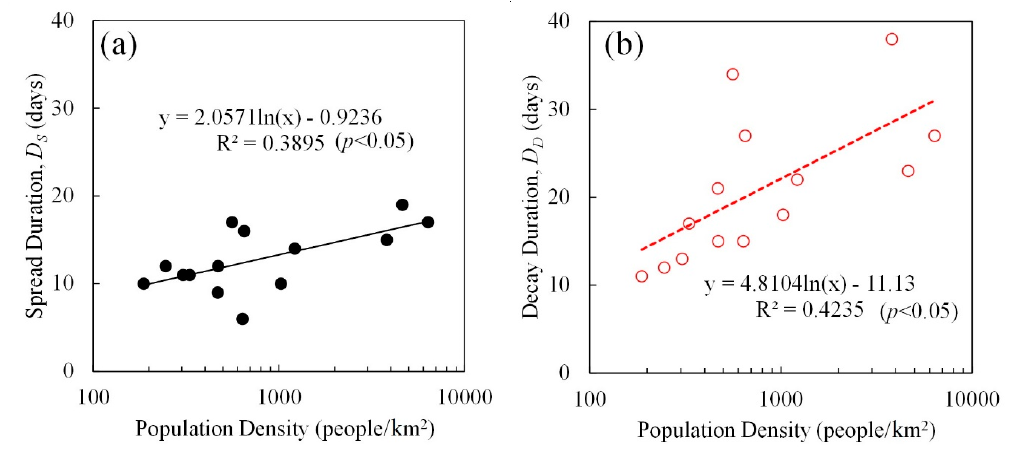
\includegraphics[width=0.8\textwidth]{0_billeder/Spread-Decay.png}
    \caption{``Relationship of the (\textbf{a}) spread and (\textbf{b}) decay duration ($D_S$ and $D_D$) with population density.'' \citep{rashed_influence_2020}}
    \label{fig:Spread-Decay}
\end{figure}
In this study, different districts in Japan with different population densities were chosen and studied, in figure \ref{fig:Spread-Decay}. The data from these districts have been plotted. There is an observable trend in this figure, which shows that population density also has a considerable effect on the spread and decay duration of COVID-19 outbreaks. 

\subsubsection{Culture}
Since it has been established that one of the main dangers of COVID-19 is how many people are gathered in a given location, cultural differences between peoples must be considered a parameter that - if nothing else - needs mentioning.

In this report, we will use the term "culture" as an umbrella term that encompasses both special occasions (Chinese New Year, American Thanksgiving etc.) and the more general way that people intermingle in their society. It should here be mentioned that scholars like Yoosefi Lebni et al. have pointed out that the cultural aspect also includes the will full endangerment of others by some people to ensure their own survival \citep{yoosefi_lebni_how_2020}. In the context of COVID-19, this cultural aspect relates specifically to hoarding and looting to ensure food and water for oneself and one's family.

Bruns et al. have pointed out that COVID-19 also greatly influenced different aspects of culture, such as greetings, major holidays and events, and interactions between family members and friendship groups \citep{bruns_covid-19_2020}. Because culture is such a vague entity, it is hard to quantify within the context of a simulation.